\chapter{子空間、投影算符與作為糾纏的測量}

貝爾定理留下了兩個問題。糾纏對中的一個成員受到擾動、被吸收或被測量後，糾纏還剩下什麼？而究竟是什麼，讓普通的相互作用成為測量？要回答這些問題，得從初等線性代數談起：性質對應子空間，機率是投影算符的期望值，而測量儀器則是另一個量子系統；物體會與它發生糾纏。

\section{開篇動機：糾纏、定域性與測量}

假設單態的兩個部分已經分隔在相距遙遠之處，其中一部分受到測量。量子場論是否必須描述它們之間的虛交換？遠處不會發生任何可探測到的事，也不會有可用的訊息傳到那裡。人們可以在局部施加磁場，旋轉其中一個自旋，改變聯合態的具體形式；但這種局部操作不會改變糾纏的量。糾纏的定量度量留待後續討論；眼前的要點是，兩個不再相互作用的系統，不會只因為一側發生了局部操作，就改變彼此共享的糾纏。

\begin{classroomqa}
\lecturetimestamp{00:00:22}
\audiencequestion{對類空分隔的單態其中一個成員進行測量，是否需要與另一個成員發生某種虛交換？}
\lecturerresponse{另一側不會發生任何可探測到的交換。局部操作可以旋轉其中一個因子，改變聯合態的表達形式，但它本身不能傳送訊息，也不能改變兩側共享的糾纏。}
\end{classroomqa}

這促使我們擴大對「夥伴」的理解。糾纏對中的一個成員若落入黑洞，另一個成員並不會因此失去糾纏；它會改與黑洞的自由度糾纏，黑洞蒸發後，則與放出的輻射糾纏。同樣的道理不必借助黑洞。把糾纏對中的一個成員丟進浴缸，讓它與水劇烈混合。它原有的個體身分可能消失在多體態中，但遠處的粒子仍與整個浴缸糾纏，最後也與逸出的水蒸氣糾纏。

這不只是糾纏如何延續的故事，也關乎可逆性。既然相互作用能產生糾纏，原則上也能解除糾纏。解糾纏是可能的，但必須讓這些系統重新接觸，再次相互作用。凡是能以一種方式發生的事，也能以相反的方式發生。

\begin{classroomqa}
\lecturetimestamp{00:04:45}
\audiencequestion{測量糾纏對的兩個自旋後，電子仍然保持糾纏嗎？一次測量就足以讓它們解糾纏嗎？}
\lecturerresponse{測量可以消除兩者之間的糾纏，而且一次測量就可能足夠。要理解這句話的含義，而不只是聲稱波函數坍縮，我們必須把觀察描述成系統與記錄儀器之間的相互作用。}
\end{classroomqa}

這個問題指出了我們的目標：把觀察、波包坍縮與糾纏連結起來。在談這個問題之前，我們需要更清楚地說明子空間與投影算符；所用的工具不會超出論證所需。

\section{維度、線性相關與正交歸一基底}

因此，我們暫時只討論配備左矢、右矢與內積的有限維向量空間。Susskind 從最基礎之處談起。他不以欄向量中的分量數目定義維度，而是抽象地將向量空間的維度定義為其中線性獨立向量的最大數目。

因此，集合 \(\{|v_i\rangle\}\) 線性獨立，意指關係式
\begin{equation}
\sum_i c_i |v_i\rangle = 0
\end{equation}
成立時，所有係數 \(c_i\) 都必須為零。換句話說，集合中的任何一個向量都不能寫成其他向量的線性組合。

這裡有一點至關重要：正交性不等於線性獨立。在三維空間中，可以有三個彼此不正交、卻線性獨立的向量。關鍵在於其中一個向量能否由另外兩個線性組合而成。另一方面，在二維平面中，任何第三個向量都必定與前兩個線性相關。

\begin{figure}[htbp]
\centering
\includegraphics[width=0.56\textwidth]{lecture_06_figure_02.png}
\caption{黑板上畫出的三個向量。講課以此草圖區分正交與線性獨立，並進一步指出，在平面中，第三個向量必定與前兩個線性相關。}
\lectureframe{00:09:35}
\end{figure}

\begin{figure}[htbp]
\centering
\begin{tikzpicture}[scale=1.2]
\draw[->] (0,0) -- (2.3,0);
\draw[->] (0,0) -- (2.0,2.0);
\draw[->] (0.35,0.95) -- (1.05,1.45);
\fill (0,0) circle (1.2pt);
\end{tikzpicture}
\caption{黑板草圖的簡化重構。單憑這一畫面無法確定確切的係數關係；幾何上的重點是，在二維平面中，第三個向量不會線性獨立。}
\end{figure}

這就是草圖要說明的重點。若空間是二維，線性獨立向量的最大數目就是二；若空間是三維，最大數目就是三。一般而言，若空間的維度為 \(d\)，在給定內積後，就能找到 \(d\) 個彼此正交的單位向量來張成該空間。這些向量就是基底向量。Susskind 明確表示，他不會在此證明這個定理；他只需要它的結論：一旦有了這樣的基底，空間中的每個向量都能以它展開。

\begin{classroomqa}
\lecturetimestamp{00:10:58}
\audiencequestion{空間自由度的數目，是否等於態空間的維度？}
\lecturerresponse{不等於。在房間中運動的粒子有三個空間座標，卻有極多彼此正交的量子態。組態空間的維度與希爾伯特空間的維度是不同的概念；此處使用有限維例子，只是為了清楚呈現其中的邏輯。}
\end{classroomqa}

\section{基底展開、並矢與恆等算符的完備性關係}

現在選取一組正交歸一基底 \(\{|n\rangle\}\)，其中 \(n=1,\dots,d\)。此時黑板上的推導尤其清楚簡潔：

\begin{figure}[htbp]
\centering
\includegraphics[width=0.62\textwidth]{lecture_06_figure_03.png}
\caption{正交歸一基底與任意態的展開。}
\lectureframe{00:14:15}
\end{figure}

我們寫成
\begin{align}
\langle m|n\rangle &= \delta_{mn}, \\
|\psi\rangle &= \sum_n a_n |n\rangle.
\end{align}
這裡 \(\delta_{mn}\) 是克羅內克符號：當 \(m=n\) 時，它等於 \(1\)；否則等於 \(0\)。

\paragraph{推導例子。}只要投影到基底向量上，就能求出各係數。從左側乘上 \(\langle m|\)：
\begin{align}
\langle m|\psi\rangle
  &= \sum_n a_n \langle m|n\rangle \\
  &= \sum_n a_n \delta_{mn} \\
  &= a_m.
\end{align}
因此，係數就是
\begin{equation}
a_m = \langle m|\psi\rangle.
\end{equation}
係數是普通的複數，放在右矢的任一側都不會改變結果。

把係數代回展開式，可得
\begin{equation}
|\psi\rangle = \sum_n |n\rangle \langle n|\psi\rangle.
\end{equation}
這表示物件 \(|n\rangle\langle n|\)，以及更一般的 \(|a\rangle\langle b|\)，應視為算符。接下來就要說明這一點。並矢的作用方式是
\begin{equation}
\bigl(|a\rangle\langle b|\bigr)|\psi\rangle = \langle b|\psi\rangle\,|a\rangle.
\end{equation}
左矢取出一個複數，右矢則給出結果向量的方向。這是 Susskind 從向量引出算符的簡明做法。

現在從算符的角度重新看前面的展開式。由於對每個 \(|\psi\rangle\) 都有
\begin{equation}
|\psi\rangle = \left(\sum_n |n\rangle\langle n|\right)|\psi\rangle
\end{equation}
括號中的算符必定是恆等算符：
\begin{equation}
\sum_n |n\rangle\langle n| = I.
\end{equation}
這就是恆等算符的完備性關係。

\begin{figure}[htbp]
\centering
\includegraphics[width=0.60\textwidth]{lecture_06_figure_07.png}
\caption{黑板上完整寫出的恆等算符完備性關係。}
\lectureframe{00:18:30}
\end{figure}

\begin{classroomqa}
\lecturetimestamp{00:18:39}
\audiencequestion{恆等算符的完備性關係中，向量必須構成一組基底嗎？}
\lecturerresponse{是的。推導同時用到了向量的歸一化與彼此正交，而且求和必須遍歷一組完備基底。任意一組向量都不能用來表示恆等算符。}
\end{classroomqa}

恆等算符本身就是投影到整個空間的投影算符。每個向量都是 \(I\) 的本徵向量，而且本徵值都是 \(+1\)。

\begin{classroomqa}
\lecturetimestamp{00:19:14}
\audiencequestion{恆等算符的完備性關係是否表示每個向量的本徵值都是一？}
\lecturerresponse{是，就恆等算符而言。它的特殊之處在於，任意向量都是它的本徵向量，而且對每個態都有 \(I|\psi\rangle=|\psi\rangle\)。}
\end{classroomqa}

\section{以子空間表示的性質與投影算符}

有了這些工具，講課便提出一項核心的概念修正：像 \(k=\lambda\) 這樣的性質一般不是單一向量，而是一整個子空間。

設 \(k\) 是厄米可觀測量，且
\begin{equation}
k|A\rangle = \lambda |A\rangle, \qquad
k|B\rangle = \lambda |B\rangle,
\end{equation}
其中 \(|A\rangle\) 與 \(|B\rangle\) 線性獨立。那麼，任何線性組合都具有相同的本徵值：
\begin{align}
k\bigl(\alpha|A\rangle+\beta|B\rangle\bigr)
  &= \alpha k|A\rangle + \beta k|B\rangle \\
  &= \alpha \lambda |A\rangle + \beta \lambda |B\rangle \\
  &= \lambda\bigl(\alpha|A\rangle+\beta|B\rangle\bigr).
\end{align}
因此，\(\lambda\) 的本徵子空間對向量相加與純量乘法封閉，是一個向量子空間。

講課中的第一個具體例子是雙自旋系統。態
\begin{equation}
|ud\rangle,\qquad |uu\rangle
\end{equation}
具有不同的第二個自旋值，但第一個自旋的值相同：兩個態中的第一個自旋都是向上。因此，它們張成第一個自旋滿足 \(\sigma_3=+1\) 的子空間。

\begin{figure}[htbp]
\centering
\includegraphics[width=0.46\textwidth]{lecture_06_figure_04.png}
\caption{第一個自旋向上的兩個雙自旋態。}
\lectureframe{00:23:27}
\end{figure}

值得保留的重點是：一項性質不一定只對應一個態，而可能涵蓋一整組具有相同本徵值的態。

為避免黑板上短暫出現的記號混淆，我們用大寫字母 \(A,B,\dots\) 表示特定的本徵向量，用小寫字母 \(a,b,\dots\) 作為求和指標，遍歷本徵子空間的一組正交歸一基底。若 \(\{|a\rangle\}\) 是子空間 \(k=\lambda\) 的一組基底，投影到該子空間的投影算符就是
\begin{equation}
\Pi_{k=\lambda}=\sum_a |a\rangle\langle a|.
\end{equation}
這只是限制在該子空間上的恆等算符。若 \(|\psi\rangle\) 已在該子空間中，投影算符會使它保持不變。若 \(|\psi\rangle\) 有一部分落在子空間之外，投影算符便會去除與子空間正交的部分，只留下其中的分量。

\section{機率公設、相容性質與貝爾定理回顧}

將性質重新理解為子空間後，機率公設便有了最簡潔的形式。若 \(|\psi\rangle\) 已歸一化，則它具有性質 \(k=\lambda\) 的機率為
\begin{equation}
P(k=\lambda)=\langle\psi|\Pi_{k=\lambda}|\psi\rangle.
\end{equation}

\begin{figure}[htbp]
\centering
\includegraphics[width=0.58\textwidth]{lecture_06_figure_05.png}
\caption{投影到 \(k=\lambda\) 本徵子空間的投影算符。黑板上的寫法已為下一步鋪路：將投影算符夾在 \(\langle\psi|\) 與 \(|\psi\rangle\) 之間。}
\lectureframe{00:31:09}
\end{figure}

代入投影算符的並矢形式：
\begin{align}
P(k=\lambda)
  &= \left\langle \psi \left| \sum_a |a\rangle\langle a| \right| \psi \right\rangle \\
  &= \sum_a \langle\psi|a\rangle\langle a|\psi\rangle \\
  &= \sum_a |\langle a|\psi\rangle|^2.
\end{align}
這正是講課中的解釋：該性質的總機率，是所有彼此正交、能使該性質成立的方式所對應機率的總和。

在雙自旋系統中，第一個自旋向上的子空間由 \(|uu\rangle\) 與 \(|ud\rangle\) 張成，因此
\begin{equation}
\Pi_{\sigma_3=+1}=|uu\rangle\langle uu|+|ud\rangle\langle ud|.
\end{equation}
講課時也會簡寫為
\begin{equation}
\Pi_{\sigma_3=+1}=\frac{1+\sigma_3}{2},
\end{equation}
其中省略了作用在第二個自旋上的恆等算符。

\begin{classroomqa}
\lecturetimestamp{00:33:04}
\audiencequestion{可觀測量、性質與投影算符有何不同？}
\lecturerresponse{可觀測量是厄米算符 \(k\)。性質 \(k=\lambda\) 由其本徵子空間表示，意指測量 \(k\) 必定得到 \(\lambda\)。投影算符 \(\Pi_{k=\lambda}\) 選出該子空間，其期望值則給出該性質成立的機率。}
\end{classroomqa}

\begin{classroomqa}
\lecturetimestamp{00:34:07}
\audiencequestion{簡併本徵向量 \(A\) 與 \(B\) 必須彼此正交嗎？它們構成整個空間的基底嗎？}
\lecturerresponse{原先的本徵向量不必彼此正交，但總能在其本徵子空間內選出一組正交歸一基底。這組基底只張成該子空間；若要張成整個空間，還需要其他正交方向。分別投影到子空間的各個基底向量上，再將結果相加，就得到投影到該子空間的投影算符。}
\end{classroomqa}

\begin{classroomqa}
\lecturetimestamp{00:35:33}
\audiencequestion{在 \(k|A\rangle=\lambda|A\rangle\) 中的符號 \(a\)，與投影算符求和中的 \(a\) 是同一種意思嗎？}
\lecturerresponse{不是。前者表示一個特定的本徵向量；求和符號下的指標則遍歷本徵子空間正交歸一基底中的所有向量。使用不同記號，便不會把固定標記誤認為求和用的虛指標。}
\end{classroomqa}

\begin{classroomqa}
\lecturetimestamp{00:37:15}
\audiencequestion{投影算符公式中的內積是機率，還是機率振幅？}
\lecturerresponse{每個 \(\langle a|\psi\rangle\) 都是機率振幅。將它乘以複共軛便得到機率；再把實現 \(k=\lambda\) 的各種彼此正交的方式所對應的機率相加，就得到該性質成立的總機率。}
\end{classroomqa}

接著，講課討論如何組合性質。假設兩項相容性質分別由彼此對易的投影算符 \(P_k\) 與 \(P_\ell\) 表示。按照講課中的說法，「且」由兩者的乘積表示：
\begin{equation}
\Pi_{k=\lambda\,\wedge\,\ell=\mu}=P_kP_\ell=P_\ell P_k.
\end{equation}
理由很簡單。\(P_k|\psi\rangle\) 位於 \(k=\lambda\) 子空間中。由於兩個算符對易，\(P_\ell P_k|\psi\rangle=P_kP_\ell|\psi\rangle\)，所以同一個向量也位於 \(\ell=\mu\) 子空間中。因此，兩者的乘積會投影到兩項性質同時成立的子空間。相應的機率為
\begin{equation}
P(k=\lambda,\ell=\mu)=\langle\psi|P_kP_\ell|\psi\rangle.
\end{equation}

值得單獨寫出這項論證的第一步。對任意態而言，
\begin{equation}
k\bigl(P_k|\psi\rangle\bigr)=\lambda P_k|\psi\rangle,
\end{equation}
因此 \(P_k|\psi\rangle\) 位於 \(k=\lambda\) 本徵子空間中。若 \(P_k\) 與 \(P_\ell\) 對易，乘積便可寫成任一投影算符置於左側的形式，因此結果同時屬於兩個子空間。

\begin{figure}[htbp]
\centering
\includegraphics[width=0.44\textwidth]{lecture_06_figure_06.png}
\caption{投影後的態，是本徵子空間中的一個向量。}
\lectureframe{00:41:57}
\end{figure}

\begin{figure}[htbp]
\centering
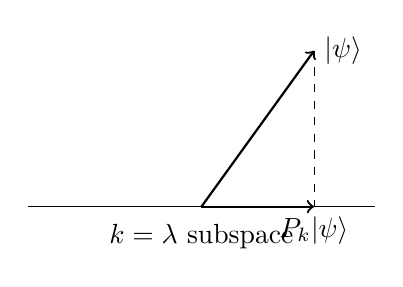
\begin{tikzpicture}[scale=1.1]
\draw (-2,0) -- (2,0);
\draw[->,thick] (0,0) -- (1.3,1.8) node[right] {$|\psi\rangle$};
\draw[dashed] (1.3,1.8) -- (1.3,0);
\draw[->,thick] (0,0) -- (1.3,0) node[below] {$P_k|\psi\rangle$};
\node at (0,-0.35) {$k=\lambda$ subspace};
\end{tikzpicture}
\caption{將任意向量投影到 \(k=\lambda\) 本徵子空間。}
\end{figure}

\begin{figure}[htbp]
\centering
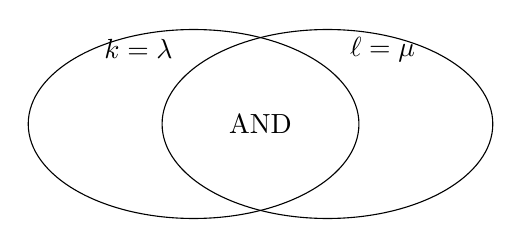
\begin{tikzpicture}[scale=1.0]
\draw (0,0) ellipse (2.1 and 1.2);
\draw (1.7,0) ellipse (2.1 and 1.2);
\node at (-0.7,0.95) {$k=\lambda$};
\node at (2.4,0.95) {$\ell=\mu$};
\node at (0.85,0) {AND};
\end{tikzpicture}
\caption{對易投影算符所代表的「且」背後，兩個子空間相交圖像的重構。}
\end{figure}

\begin{figure}[htbp]
\centering
\includegraphics[width=0.66\textwidth]{lecture_06_figure_08.png}
\caption{黑板上的論證：對易投影算符選出同時本徵子空間。}
\lectureframe{00:45:20}
\end{figure}

\begin{classroomqa}
\lecturetimestamp{00:44:42}
\audiencequestion{同時成立的性質，是否就等於經典邏輯中的交集？}
\lecturerresponse{是。對易投影算符的乘積 \(P_kP_\ell\) 會投影到兩個本徵子空間的交集。若交集只有零向量，就沒有非零態能同時具有這兩項性質。}
\end{classroomqa}

完整起見，相容的「或」子空間所對應的投影算符為
\begin{equation}
P_{k\lor\ell}=P_k+P_\ell-P_kP_\ell .
\end{equation}
若兩種可能互斥，則 \(P_kP_\ell=0\)，上式便化為總和 \(P_k+P_\ell\)。只要兩個子空間有所重疊，就必須做這項減法，才能避免把交集計算兩次。

接著，講課以具體物理例子說明相容性。在雙自旋系統中，第一個自旋的任意分量 \(\sigma_i\) 都與第二個自旋的任意分量 \(\tau_j\) 對易：
\begin{equation}
[\sigma_i,\tau_j]=0.
\end{equation}
相較之下，同一個自旋的不同分量彼此不對易：
\begin{equation}
[\sigma_1,\sigma_3]\neq 0.
\end{equation}
因此，可以分別測量兩個分離自旋的某一分量，卻不能同時測量同一個自旋的兩個不同分量。

\begin{classroomqa}
\lecturetimestamp{00:46:12}
\audiencequestion{相容可觀測量有哪些具體例子？}
\lecturerresponse{作用在第一個自旋上的任何算符，都與作用在第二個自旋上的任何算符對易，因為兩者作用於不同的張量因子。位置分量 \(x,y,z\) 也是一組彼此相容的可觀測量。相較之下，同一自旋的兩個不同分量，以及位置與其共軛動量，都不對易。}
\end{classroomqa}

\begin{classroomqa}
\lecturetimestamp{00:47:26}
\audiencequestion{子系統一定得是不同的粒子嗎？}
\lecturerresponse{不一定。子系統指的是一組獨立指定的自由度。不同粒子提供最簡單的張量因子；若算符結構允許，同一粒子的不同自由度也能分開處理。}
\end{classroomqa}

\begin{classroomqa}
\lecturetimestamp{00:48:37}
\audiencequestion{不同子系統上的算符既然常常對易，那麼簡單的不相容例子是什麼？}
\lecturerresponse{同一個自旋的兩個分量是典型例子：\(\sigma_1\) 與 \(\sigma_3\) 不對易，因此沒有任何儀器能同時為兩者指定確定值。矩陣對易子不為零，就是代數上的判據。}
\end{classroomqa}

現在 Susskind 重新檢視貝爾定理。他不再重算上一講的數值，而是用新的語言重建其中的邏輯。經典不等式以機率形式寫成
\begin{equation}
P(A\wedge \neg B)+P(B\wedge \neg C)\ge P(A\wedge \neg C).
\end{equation}
這是經典集合邏輯的定理，不是量子力學的定理。在單態中，自旋沿任何共同軸都反向排列，因此可以把「第一個自旋不具有某性質」換成「第二個自旋具有相應性質」的陳述。如此便能將不等式改寫為關於雙自旋系統聯合性質的陳述。

略去未作用因子上的恆等算符後，講課中出現的單一性質投影算符為
\begin{equation}
\frac{1+\sigma_3}{2},\qquad
\frac{1+\frac{\tau_1+\tau_3}{\sqrt2}}{2},\qquad
\frac{1+\frac{\sigma_1+\sigma_3}{\sqrt2}}{2},\qquad
\frac{1+\tau_1}{2}.
\end{equation}
因此，三個相關的聯合投影算符為
\begin{align}
\Pi_1 &= \frac{1+\sigma_3}{2}\,\frac{1+\frac{\tau_1+\tau_3}{\sqrt2}}{2}, \\
\Pi_2 &= \frac{1+\frac{\sigma_1+\sigma_3}{\sqrt2}}{2}\,\frac{1+\tau_1}{2}, \\
\Pi_3 &= \frac{1+\sigma_3}{2}\,\frac{1+\tau_1}{2}.
\end{align}

\begin{figure}[htbp]
\centering
\includegraphics[width=0.68\textwidth]{lecture_06_figure_09.png}
\caption{三種分析器設定，以單自旋投影算符的乘積表示。}
\lectureframe{01:01:45}
\end{figure}

講課以熟悉的黑板寫法談到未歸一化的單態
\begin{equation}
|\Psi_{\mathrm{singlet}}\rangle \propto |ud\rangle-|du\rangle.
\end{equation}
在此，比例符號已經足夠。對論證而言，重要的是態本身，尤其是相對符號，而不是整體的歸一化。在單態中計算 \(\langle \Pi_1\rangle+\langle \Pi_2\rangle\) 與 \(\langle \Pi_3\rangle\)，會得到上一講所推導的違反結果。Susskind 口頭強調的結論是：量子力學並非偽裝成經典集合論。

\begin{classroomqa}
\lecturetimestamp{00:52:31}
\audiencequestion{若自旋向上與自旋向下彼此正交，負號是否表示其中一個右矢是另一個的負值？}
\lecturerresponse{不是。\(|u\rangle\) 與 \(|d\rangle\) 是不同且彼此正交的向量。相對符號屬於 \(|ud\rangle-|du\rangle\) 這類疊加態，會影響其物理性質；只有乘在整個態上的整體符號才不具物理影響。}
\end{classroomqa}

\begin{classroomqa}
\lecturetimestamp{00:53:06}
\audiencequestion{量子態和性質的每一種選擇，都會違反貝爾不等式嗎？}
\lecturerresponse{不會。許多態與許多軸的選擇，都會符合某個特定的貝爾不等式。是否違反，取決於態以及所選的可觀測量。改變中間角度與末端角度，會影響這項檢驗能否揭露非經典關聯。}
\end{classroomqa}

\begin{classroomqa}
\lecturetimestamp{01:02:47}
\audiencequestion{某個特定態違反或恰好符合這項貝爾不等式時，可以得出什麼結論？}
\lecturerresponse{違反不等式，證明觀測到的統計結果不可能來自推導中採用的經典集合邏輯。符合某一選定的不等式，並不能單憑此點判定該態是經典的，因為改選其他性質仍可能揭露違反。}
\end{classroomqa}

\section{貝爾定理之後的定域性}

投影算符的計算不只是符號遊戲。設想反覆製備處於單態基態的關聯粒子對，將每對粒子的兩個成員分開，再把這些以相同方式製備的粒子對分成三大組。第一組測量 \(0^\circ\) 與 \(45^\circ\) 的設定，第二組測量 \(45^\circ\) 與 \(90^\circ\) 的設定，第三組測量 \(0^\circ\) 與 \(90^\circ\) 的設定。三組測得的頻率可用來估計不等式中的三個機率。

\begin{classroomqa}
\lecturetimestamp{01:04:30}
\audiencequestion{三個貝爾機率實際描述的是什麼樣的實驗室安排？}
\lecturerresponse{一個來源產生許多以相同方式製備的糾纏粒子對，並將每對的兩個成員送往相隔甚遠的分析器。把粒子對分成三組，並在每組使用相應的一對分析器方向。統計聯合測量結果，即可估計各項機率。帶電粒子與反粒子可以藉由場分開；實際的貝爾實驗則常使用光子。}
\end{classroomqa}

\begin{classroomqa}
\lecturetimestamp{01:08:00}
\audiencequestion{經典集合論的證明使用同一個母體，三組分別測量的樣本如何檢驗這項證明？}
\lecturerresponse{這個不等式談的不只是計數，也談機率。若三組樣本都來自相同的製備程序，其相對頻率便能估計同一共同系綜中的三個機率分布。製備方式相同是不可或缺的假設。}
\end{classroomqa}

回顧貝爾定理後，講課便直接回到那個仍令人不安的物理問題：如果這些關聯真實存在，為什麼不能用它們傳送訊號？

\begin{classroomqa}
\lecturetimestamp{01:09:41}
\audiencequestion{為什麼不能利用糾纏關聯傳送超光速訊息？}
\lecturerresponse{單獨觀察任一側，看到的仍是無法控制的隨機序列。只有透過一般的古典通訊通道比對兩側的紀錄，才能看出其中的關聯。決定性的貝爾實驗會安排測量設定與探測時序，使光訊號來不及在兩側之間傳遞，因而排除以定域通訊機制產生聯合統計結果的可能。}
\end{classroomqa}

如果光訊號有足夠時間在裝置之間傳播，關聯本身並不違反相對論；我們可能只是發現了先前未察覺的一般影響。嚴格的實驗會封住這條退路。用貝爾的說法，能重現這些關聯的隱變數描述必須是非定域的；但非定域的依賴關係不等於可控制的超光速訊息。

\begin{classroomqa}
\lecturetimestamp{01:12:18}
\audiencequestion{角動量守恆是這項論證不可或缺的條件嗎？}
\lecturerresponse{不是。自旋只是方便的二態模型，並非不可或缺的要素。只要一對二能級系統具有所需的糾纏態與不同的測量基底，就能呈現相同的邏輯結構。}
\end{classroomqa}

這段討論並未結束講課，而是為下一個轉折鋪路。貝爾定理讓我們知道，量子力學並非經典邏輯；接下來要問的是另一個問題：從操作與數學的角度來看，測量究竟是什麼？它如何參與干涉？

\section{有限態雙狹縫、干涉與作為糾纏的測量}

講課現在換了一個模型。Susskind 轉向雙狹縫實驗，隨即將它簡化為有限態問題，好讓我們沿用相同的向量空間方法，而不必引入連續波動力學的完整架構。他的意思是，這仍然是雙狹縫實驗，只是把它簡化成一小組基底態。

這裡有一個源態 \(|0\rangle\)、兩個狹縫態 \(|1\rangle\) 與 \(|-1\rangle\)，以及一組屏幕態 \(|n\rangle\)。這些 \(|n\rangle\) 彼此正交，因為不同的屏幕位置代表不同的組態。講課明確表示，此處暫且不仔細追蹤歸一化，並將么正性留待後續處理。這個階段的重點是線性。

\begin{figure}[htbp]
\centering
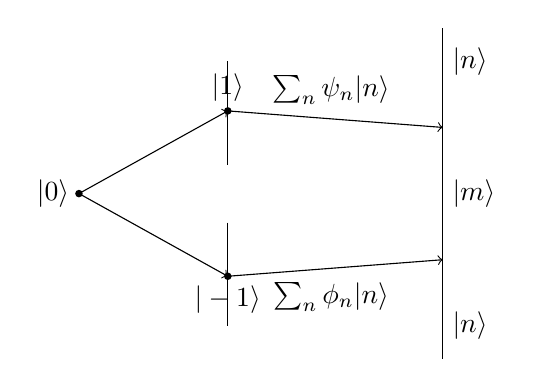
\begin{tikzpicture}[scale=1.05]
\fill (0,0) circle (1.3pt);
\node[left] at (0,0) {$|0\rangle$};

\draw (1.8,1.6) -- (1.8,0.35);
\draw (1.8,-0.35) -- (1.8,-1.6);
\fill (1.8,1) circle (1.3pt);
\fill (1.8,-1) circle (1.3pt);
\node[above] at (1.8,1) {$|1\rangle$};
\node[below] at (1.8,-1) {$|-1\rangle$};

\draw (4.4,2.0) -- (4.4,-2.0);
\node[right] at (4.4,1.6) {$|n\rangle$};
\node[right] at (4.4,0.0) {$|m\rangle$};
\node[right] at (4.4,-1.6) {$|n\rangle$};

\draw[->] (0,0) -- (1.8,1);
\draw[->] (0,0) -- (1.8,-1);
\draw[->] (1.8,1) -- (4.4,0.8);
\draw[->] (1.8,-1) -- (4.4,-0.8);

\node at (3.05,1.25) {$\sum_n \psi_n |n\rangle$};
\node at (3.05,-1.25) {$\sum_n \phi_n |n\rangle$};
\end{tikzpicture}
\caption{有限態雙狹縫實驗：源態 \(|0\rangle\)、兩個狹縫態 \(|1\rangle\) 與 \(|-1\rangle\)，以及屏幕基底 \(|n\rangle\)。}
\end{figure}

\begin{figure}[htbp]
\centering
\includegraphics[width=0.68\textwidth]{lecture_06_figure_10.png}
\caption{有限位置晶格，以及線性演化規則 \(A\to A'\)、\(B\to B'\)。}
\lectureframe{01:18:00}
\end{figure}

由對稱性可知，源態會演化為兩個狹縫態的等振幅疊加：
\begin{equation}
|0\rangle \longrightarrow |1\rangle+|-1\rangle.
\end{equation}
接著，令上狹縫態演化為
\begin{equation}
|1\rangle \longrightarrow \sum_n \psi_n |n\rangle,
\end{equation}
並令下狹縫態演化為
\begin{equation}
|-1\rangle \longrightarrow \sum_n \phi_n |n\rangle.
\end{equation}
這些箭頭表示時間演化，而不是說同一時刻的兩個態相等。根據線性，
\begin{equation}
|1\rangle+|-1\rangle \longrightarrow \sum_n (\psi_n+\phi_n)|n\rangle.
\end{equation}
這就是關鍵規則：先將振幅相加，再計算機率。

\begin{classroomqa}
\lecturetimestamp{01:21:59}
\audiencequestion{狹縫處的態 \(|1\rangle\) 怎麼會演化成同樣以整數 \(n\) 標記的態？這些右矢描述的是同一地點、同一時間嗎？}
\lecturerresponse{這些標記指的是不同的時間切片。\(|1\rangle\)表示電子位於上狹縫；右邊的 \(|n\rangle\) 則表示電子之後可能出現在螢幕上的位置。箭頭表示時間演化，並不表示同一時間的不同組態彼此相等。}
\end{classroomqa}

\begin{classroomqa}
\lecturetimestamp{01:25:30}
\audiencequestion{振幅需要歸一化嗎？振幅有物理單位嗎？}
\lecturerresponse{完整的演化必須保持總機率不變，這就是么正性。這裡省略了共同的歸一化因子，因為我們只關心路徑振幅的相加與相消。將態歸一化時，可以再補回任何比例因子。}
\end{classroomqa}

因此，到達螢幕位置 \(m\) 的機率為
\begin{align}
P_m &= |\psi_m+\phi_m|^2 \\
    &= |\psi_m|^2 + |\phi_m|^2 + \psi_m^*\phi_m + \phi_m^*\psi_m.
\end{align}
前兩項是經典推理會得到的結果，後兩項則是干涉項。

\begin{figure}[htbp]
\centering
\includegraphics[width=0.68\textwidth]{lecture_06_figure_11.png}
\caption{黑板上的螢幕振幅及其展開成四項的機率。}
\lectureframe{01:29:20}
\end{figure}

在螢幕上的對稱位置，也就是 \(m=0\)，由對稱性可知 \(\psi_0=\phi_0\)。於是
\begin{equation}
P_0 = |\psi_0+\phi_0|^2 = |2\psi_0|^2 = 4|\psi_0|^2.
\end{equation}
在該位置，雙狹縫同時開啟時的機率是單一狹縫開啟時的四倍，而非兩倍。這是相長干涉。

現在加入相移，使得 \(\phi_0=-\psi_0\)。於是
\begin{equation}
P_0 = |\psi_0-\psi_0|^2 = 0.
\end{equation}
任一狹縫單獨開啟時，電子都可能到達該位置；但兩個狹縫同時開啟時，電子卻可能完全無法到達那裡。這是相消干涉。Susskind 特別強調這有多麼奇怪：在他看來，這跟 Bell 的情況一樣奇怪。

\begin{classroomqa}
\lecturetimestamp{01:33:14}
\audiencequestion{如果等電子已經在飛行途中，才改變相移器或狹縫的選擇，會怎麼樣？另一個狹縫需要時間才會知道這項改變嗎？}
\lecturerresponse{答案取決於具體的時空安排，也取決於電子是否會遇到裝置中被改動的部分。量子力學描述態如何經過實際裝置演化；機率仍由相關振幅相加而得。要評估局域性方面的主張，就必須明確界定延遲選擇方案。}
\end{classroomqa}

現在引入裝置。另有一個二態系統，也就是一個自旋，最初處於態 \(|d\rangle\)。電子若穿過上狹縫，自旋便翻轉為 \(|u\rangle\)；若穿過下狹縫，自旋則保持不變。初始複合態為 \(|0,d\rangle\)，第一條更新規則因此變為
\begin{equation}
|0,d\rangle \longrightarrow |1,u\rangle + |-1,d\rangle.
\end{equation}
這一行就概括了講座中測量的全部含義：電子的位置已與裝置中儲存的記錄糾纏。

\begin{figure}[htbp]
\centering
\includegraphics[width=0.66\textwidth]{lecture_06_figure_12.png}
\caption{探測器自旋將其向上與向下的記錄分別和兩種狹縫選擇關聯起來。}
\lectureframe{01:44:10}
\end{figure}

\begin{classroomqa}
\lecturetimestamp{01:40:20}
\audiencequestion{兩個狹縫都需要設置探測器嗎？}
\lecturerresponse{一個可靠的探測器就足夠了。如果探測器記錄到電子穿過上狹縫，那麼記錄未改變就表示電子走的是下狹縫；前提是每個透射的電子都必須穿過兩個開口之一。也可以設置第二個探測器，但這只會多加入一個子系統，並不會改變原理。}
\end{classroomqa}

\begin{classroomqa}
\lecturetimestamp{01:40:51}
\audiencequestion{為什麼不說電子同時穿過兩個狹縫？}
\lecturerresponse{沒有路徑記錄時，態是相干疊加，無法回頭判定電子實際走過哪條路徑。若進行完整的路徑測量，裝置便會在每次實驗中記錄其中一種選擇。兩種選擇都保有的是態振幅，而不是兩條分別觀測到的電子軌跡。}
\end{classroomqa}

\begin{figure}[htbp]
\centering
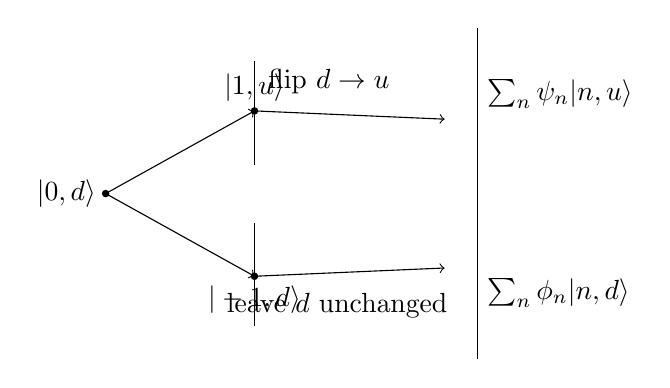
\begin{tikzpicture}[scale=1.05]
\fill (0,0) circle (1.3pt);
\node[left] at (0,0) {$|0,d\rangle$};

\draw (1.8,1.6) -- (1.8,0.35);
\draw (1.8,-0.35) -- (1.8,-1.6);
\fill (1.8,1) circle (1.3pt);
\fill (1.8,-1) circle (1.3pt);
\node[above] at (1.8,1) {$|1,u\rangle$};
\node[below] at (1.8,-1) {$|-1,d\rangle$};

\draw (4.5,2.0) -- (4.5,-2.0);
\node[right] at (4.5,1.2) {$\sum_n \psi_n |n,u\rangle$};
\node[right] at (4.5,-1.2) {$\sum_n \phi_n |n,d\rangle$};

\draw[->] (0,0) -- (1.8,1);
\draw[->] (0,0) -- (1.8,-1);
\draw[->] (1.8,1) -- (4.1,0.9);
\draw[->] (1.8,-1) -- (4.1,-0.9);

\node at (2.7,1.35) {flip \(d\to u\)};
\node at (2.8,-1.35) {leave \(d\) unchanged};
\end{tikzpicture}
\caption{測量可視為與探測器自旋的糾纏：上方路徑會翻轉裝置自旋，下方路徑則讓自旋保持不變。}
\end{figure}

假設如講座中所述，自旋在前往螢幕的途中不再發生任何變化。於是
\begin{align}
|1,u\rangle &\longrightarrow \sum_n \psi_n |n,u\rangle, \\
|-1,d\rangle &\longrightarrow \sum_n \phi_n |n,d\rangle.
\end{align}
因此，雙狹縫都開啟時的末態為
\begin{equation}
|\Psi_{\mathrm{final}}\rangle
  = \sum_n \psi_n |n,u\rangle + \sum_n \phi_n |n,d\rangle.
\end{equation}
這不是單一電子自身的疊加態，而是電子與裝置的糾纏態。

\begin{figure}[htbp]
\centering
\includegraphics[width=0.68\textwidth]{lecture_06_figure_13.png}
\caption{兩條路徑的振幅抵達螢幕時，各自帶有彼此正交的裝置記錄。}
\lectureframe{01:47:35}
\end{figure}

計算電子到達位置 \(m\) 的機率，最直接的方法是在電子子系統上使用投影至該位置的投影算符：
\begin{equation}
\Pi_m = |m\rangle\langle m|\otimes I_{\mathrm{spin}}.
\end{equation}
將 \(\Pi_m\) 作用於末態，得到
\begin{equation}
\Pi_m |\Psi_{\mathrm{final}}\rangle
= |m\rangle\bigl(\psi_m|u\rangle+\phi_m|d\rangle\bigr).
\end{equation}
因此，到達位置 \(m\) 的機率為
\begin{align}
P_m
  &= \langle \Psi_{\mathrm{final}}|\Pi_m|\Psi_{\mathrm{final}}\rangle \\
  &= \bigl(\psi_m^*\langle u|+\phi_m^*\langle d|\bigr)
     \bigl(\psi_m|u\rangle+\phi_m|d\rangle\bigr) \\
  &= |\psi_m|^2 + |\phi_m|^2
     + \psi_m^*\phi_m\langle u|d\rangle
     + \phi_m^*\psi_m\langle d|u\rangle.
\end{align}
但記錄態彼此正交：
\begin{equation}
\langle u|d\rangle=0.
\end{equation}
因此交叉項消失：
\begin{equation}
P_m = |\psi_m|^2 + |\phi_m|^2.
\end{equation}
這就是講座中的數學要點。一旦路徑資訊被記錄下來，干涉就會消失，機率便如經典情況般相加。

\begin{classroomqa}
\lecturetimestamp{01:49:09}
\audiencequestion{疊加態 \(|1\rangle+|-1\rangle\) 和態 \(|1,u\rangle+|-1,d\rangle\) 有什麼不同？}
\lecturerresponse{前者描述單一系統處於兩個位置的線性組合，沒有其他系統可與它糾纏。後者則涉及兩個系統，將路徑和探測器自旋關聯起來。讀取自旋就能得知路徑資訊。}
\end{classroomqa}

\section{環境記錄與部分測量}

刻意設置的探測器並非唯一能留下記錄的事物。狹縫附近的原子、殘餘氣體、熱表面，或任何其他自由度，都可能與路徑產生關聯。若其末態為 \(|E_1\rangle\) 和 \(|E_2\rangle\)，路徑態便具有以下形式：
\begin{equation}
|\Psi\rangle
=\sum_n\left(\psi_n|n\rangle|E_1\rangle
+\phi_n|n\rangle|E_2\rangle\right).
\end{equation}
此時干涉項會乘上重疊量 \(\langle E_1|E_2\rangle\)。正交的記錄能讓兩條路徑完全可區分，干涉也就完全消失。記錄相同時，\(\langle E_1|E_2\rangle=1\)，干涉便得以保留。重疊程度介於兩者之間時，可見度也介於兩者之間。

\begin{figure}[htbp]
\centering
\includegraphics[width=0.68\textwidth]{lecture_06_figure_14.png}
\caption{彼此重疊與分離的環境波包，分別呈現部分與完整的路徑記錄。}
\lectureframe{01:53:40}
\end{figure}

\begin{classroomqa}
\lecturetimestamp{01:50:48}
\audiencequestion{即使沒有人刻意觀測，狹縫附近的一般原子也會與經過的電子糾纏嗎？}
\lecturerresponse{會。關鍵不在於「知道」，而在於是否產生物理關聯。若原子或周圍氣體受到足夠擾動，使其後來的狀態能區分電子走過哪條路徑，它就會留下路徑資訊，並抑制干涉。這就是此類實驗需要隔離、低溫，且常使用光子等交互作用較弱的粒子的原因。}
\end{classroomqa}

冷卻會使環境自由度接近基態，減少意外留下的記錄。能隙也有幫助：若入射粒子無法提供最低激發所需的能量，環境便可能無法留下路徑資訊。反過來說，帶電粒子會透過電場擾動附近物質，因此電子干涉實驗尤其難以進行。

\begin{classroomqa}
\lecturetimestamp{01:54:49}
\audiencequestion{真的能用單顆電子得到干涉圖樣嗎？}
\lecturerresponse{每顆電子只會在一處留下局域的撞擊。讓電子一次通過一顆，彼此間隔足夠遠以避免交互作用，再重複收集大量事件。累積的頻率分布會呈現干涉圖樣；單一事件只是一個小點。}
\end{classroomqa}

\begin{classroomqa}
\lecturetimestamp{01:55:59}
\audiencequestion{測量會破壞糾纏，還是產生糾纏？}
\lecturerresponse{路徑測量中的交互作用會使系統與裝置糾纏，而這種糾纏會破壞不同選擇之間的干涉。後續測量可以使裝置與另一個系統產生關聯，也可能對剩餘態施加條件。因此，必須明確指出討論的是哪兩個子系統，以及哪一種干涉。}
\end{classroomqa}

\begin{classroomqa}
\lecturetimestamp{01:57:44}
\audiencequestion{能否減弱交互作用，讓裝置只取得部分路徑資訊？}
\lecturerresponse{可以。弱交互作用可能只以一定振幅翻轉探測器，使記錄態保持非正交。如此一來，兩條路徑只有部分可區分，干涉也只會部分減弱。測量越強，路徑越容易區分，裝置與記錄的糾纏越強，條紋可見度則越低。}
\end{classroomqa}

因此，這裡所說的坍縮有具體意義：路徑資訊被留在另一個系統中時，交叉項便會消失。沒有記錄時，振幅相加；記錄完全可區分時，它們的內積為零，機率相加。在這兩個極端之間，測量強度與干涉可見度會連續變化。